\chapter{Constraining {\sc Galacticus}}

\section{Model Accuracy}\label{sec:ModelAccuracy}

The model accuracy script processes the model described by a standard \glc\ constraints configuration file to assess how accurate the model is. Specifically, it determines the relative contribution to the covariance of each constraint arising from the finite number of merger trees run in the model and the intrinsic covariance of the observations. An accurate model should make a negligible contribution to the covariance.

To run the model accuracy script use
\begin{verbatim}
 constraints/testModelAccuracy.pl <configFile>
\end{verbatim}
where {\tt configFile} is the name of the configuration file. The script will run the model multiple times, reducing the number of trees per decade by a factor of two each time (this is done 8 times, such that the smallest model run has a factor 128 times fewer trees than the original model). Furthermore, this sequence of models is run for three different choices for sampling halo masses: {\tt powerLaw}, {\tt haloMassFunction}, and {\tt stellarMassFunction} (see \S\ref{sec:MassSamplingDensityFunction}).

For each constraint in the specified constraint compilation and accuracy measure is constructed which is the root mean squared ratio of the error arising from the finite number of trees and the intrinsic error of the constraint data. 

Accuracy analysis files are written to:
\begin{verbatim}
 <workDirectory>/accuracy
\end{verbatim}
For each constraint in the compilation a plot showing accuracy measure as a function of CPU time is written to
\begin{verbatim}
 <constraintLabel>_mergerTreeBuildTreesPerDecade.pdf
\end{verbatim}
Each point in the plot is labelled with the number of merger trees per decade. An accurate model should have accuracy measure significantly below unity. This plot is also useful to see which sampling method achieves that accuracy in the least amount of CPU time.

Additionally, a report is written to:
\begin{verbatim}
 <constraintLabel>Report.txt
\end{verbatim}
This file lists, for each sampling method, the accuracy measure achieved and the CPU time taken for the largest model run.

\section{Model Convergence}\label{sec:ModelConvergence}

The model convergence script processes the model described by a standard \glc\ constraints configuration file to assess how well converged the model is with respect to several of \glc's numerical parameters. Specifically, it determines the a covariance measure for each constraint in the specified compilation file.

To run the model convergence script use
\begin{verbatim}
 constraints/testConvergnce.pl <configFile>
\end{verbatim}
where {\tt configFile} is the name of the configuration file. The script will run the model multiple times, adjusting the value of a numerical parameter each time.

For each constraint in the specified constraint compilation a convergence measure, $C$, is constructed which
\begin{equation}
 C = \sum_i {(y_i - y_{{\rm ideal}, i})^2 \over \sqrt{2} \sigma_{{\rm ideal}, i}^2}
\end{equation}
where $y_i$ is the result of the constraint, $\sigma_i$ is the error on the result, and subscript ``ideal'' refers to the model with the most ideal value (i.e. that in the original, unmodified model) of the numerical parameter being tested (which might be the lowest value for a mass resolution, or the highest value for the maximum tree mass simulated for example). To be converged, the convergence measure should remain consistent with unity within a significant distance\footnote{``Significant distance'' here requires some judgement. Typically we would like for the model results to not change significantly as the value of a numerical parameter is adjusted by at least a factor of 2 away from the ideal value.} away from the ideal value.

Convergence analysis files are written to:
\begin{verbatim}
 <workDirectory>/convergence
\end{verbatim}
For each combination of constraint in the compilation and numerical parameter a plot showing the convergence measure as a function of the numerical parameter is created in:
\begin{verbatim}
 <constraintLabel>_<numericalParameter>.pdf
\end{verbatim}
Each point in the plot has an error bar since, due to the limited number of merger trees run, the convergence measure is not known with perfect precision. A horizontal line shows the desired convergence measure of unity.

Additionally, a report is written to:
\begin{verbatim}
 <constraintLabel>Report.txt
\end{verbatim}
This file lists, for each numerical parameter, the convergence measure and its error achieved by the ideal model. Additionally a normalized measure (the measure divided by its error) is listed. This normalized measure can be approximately interpretted as the number of $\sigma$ deviation from convergence.

\section{Model Discrepancy}\label{sec:ModelDiscrepancy}

Model discrepancy scripts process the model described by a standard \glc\ constraints configuration file to produce an output HDF5 file which describes a particular contribution to the model discrepancy. The format of these files is
\begin{verbatim}
HDF5 "discrepancy.hdf5" {
GROUP "/" {
   DATASET "additive" {
   }
   DATASET "multiplicative" {
   }
   DATASET "covariance" {
   }
}
\end{verbatim}
Each of the three datasets is optional (i.e. not all need be provided for each discrepancy). The {\tt additive} dataset gives an additive offset which will be applied to the relevant model results. The {\tt multiplicative} dataset similarly gives a multiplicative offset which will be applied to the relevant model results. Finally, the {\tt covariance} dataset gives the contribution from this discrepancy to the covariance matrix used in evaluating the model likelihood.

Discrepancy files are written to
\begin{verbatim}
 <workDirectory>/modelDiscrepancy/<discrepancyLabel>/discrepancy<constraintLabel>.hdf5
\end{verbatim}

Constraint scripts (see \S\ref{sec:ConstraintScripts}) accept a command line option {\tt --modelDiscrepancies} which specifies the path to the {\tt modelDiscrepancy} directory (i.e. {\tt <workDirectory>/modelDiscrepancy}) and will search for any relevant model discrepancy files and apply them in their calculations.

\subsection{Monte Carlo Merger Trees}

\glc\ typically uses Monte Carlo-generated merger trees when being constrained to fit data. These have the advantage that they can be generated for any cosmological parameters (necessary if the cosmological parameters are to be varied as part of the constraining process) and they can be generated uniquely for each model evaluation which avoids any bias introduced by using a fixed set of halos.

However, these Monte Carlo-generated trees may not precisely capture the properties of merger trees derived from a fully non-linear calculation of gravitational collapse (e.g. as performed by an N-body simulation). Therefore it is important to assess the model discrepancy arising from this limitation.

Model discrepancy files can be generated using:
\begin{verbatim}
 constraints/modelDiscrepancy/monteCarloTrees.pl config.xml
\end{verbatim}
where {\tt config.xml} is a standard \glc\ constraint configuration file. The script will run two sets of models, one using N-body merger trees derived from the \gls{millenniumSimulation}, and a second using Monte Carlo-generated merger trees. The number of subvolumes of the \gls{millenniumSimulation} to use is specified by the {\tt subVolumeCount} option to this script (a default of $32$ subvolumes is used if no number is specified). The subvolume data will be downloaded from the \gls{millenniumSimulation} database if necessary.

To make a fair comparison, \gls{millenniumSimulation} merger trees have their branches pruned below a mass corresponding to $20$ particles, and the Monte Carlo merger trees are built with the equivalent mass resolution. Additionally, the Monte Carlo merger trees are regridded onto a set of timesteps matched to the \gls{millenniumSimulation}.

A multiplicative model discrepancy is computed for each constraint included in the compilation (as specified in the configuration file) equal to the ratio of the N-body result to the Monte Carlo result. Additionally, the subvolumes of the \gls{millenniumSimulation} are used to estimate the covariance in the N-body result due to the finite volume of the simulation. The result is computed for each subvolume separately and the covariance of the result between subvolumes computed. This is repeated using pairs of subvolumes, quads of subvolumes, etc. If $2^n$ subvolumes were used, then the covariance measured from the result combining $2^{n-3}$ subvolumes is used to extrapolate the covariance for all $512$ subvolumes assuming that the covariance scales in inverse proportion to the number of subvolume used. Finally, the contribution of the Monte Carlo trees model to the covariance is assumed to be a diagonal matrix with elements equal to the square of the reported errors on the result of the model.

\subsection{Fixed Virial Orbits}

The orbital parameters of subhalos at the point of virial orbit crossing are usually drawn from an appropriate cosmological distribution. If instead fixed virial orbital parameters are used instead then term should be included in the model discrepancy accounting for this approximation. 

Model discrepancy files can be generated using:
\begin{verbatim}
 constraints/modelDiscrepancy/fixedVirialOrbits.pl config.xml
\end{verbatim}
where {\tt config.xml} is a standard \glc\ constraint configuration file. The script will run two models, one using fixed virial orbital parameters, and a second using variable orbital parameters using the {\tt Benson2005} method (see \S\ref{sec:VirialOrbitsBenson2005}). A multiplicative model discrepancy is computed for each constraint included in the compilation (as specified in the configuration file) equal to the ratio of the variable orbits result to the fixed orbits result. Additionally, a model discrepancy covariance is computed. This is assumed to be a diagonal matrix with elements equal to the square of the reported errors on the results of the fixed and variable orbital parameters models.

\subsection{Jiang et al. (2008) Merger Time Scatter}

The \cite{jiang_fitting_2008} algorithm for the merging times of dark matter subhalos includes drawing times from a log-normal distribution of width $\sigma=0.4$ with median equal to their fitting function (see \S\ref{sec:DynamicalFrictionJiang2008}). If instead zero scatter is used then a term should be included in the model discrepancy accounting for this approximation. 

Model discrepancy files can be generated using:
\begin{verbatim}
 constraints/modelDiscrepancy/jiang2008MergingTimeScatter.pl config.xml
\end{verbatim}
where {\tt config.xml} is a standard \glc\ constraint configuration file. The script will run two models, one using the default scatter specified by the configuration file, and a second using $\sigma=0.4$. A multiplicative model discrepancy is computed for each constraint included in the compilation (as specified in the configuration file) equal to the ratio of the $\sigma=0.4$ and default scatter results. Additionally, a model discrepancy covariance is computed. This is assumed to be a diagonal matrix with elements equal to the sum of the square of the reported errors on the result of the default scatter and $\sigma=0.4$ models.

\section{Optimal Halo Mass Function Sampling}

Suppose we want to fit parameters of the \glc\ model to some dataset. The basic approach is to generate large numbers of model realizations for different parameter values and see which ones best match the data. \glc\ models involve simulating individual merger trees and then adding together their galaxies to produce some overall function. The question we want to answer is, given some finite amount of computing time, what is the optimal distribution of halo masses to run when comparing to a given dataset. For example, is it better to run a volume limited sample (as one would get from an N-body simulation) or is it better to use, say, equal numbers of halos per logarithmic interval of halo mass? The following section describes how to solve this optimization problem in the specific case of fitting to the stellar mass function.

\subsection{Li \& White (2009) Stellar Mass Function}\label{sec:OptimalSamplingStellarMassFunction}

First, some definitions:
\begin{description}
 \item [$n(M) \d \ln M$] is the dark matter halo mass function, i.e. the number of halos in the range $M$ to $M+M\d\ln  M$ per unit volume;
 \item [$\gamma(M) \d \ln M$] is the number of trees that we will simulate in the range $M$ to $M+M\d \ln M$;
 \item [$\alpha(M_\star)$] is the error on the observed stellar mass function at mass $M_\star$;
 \item [$P(N|M_\star,M;\delta \ln M_\star)$] is the conditional stellar mass distribution function of galaxies of stellar mass $M_\star$ in a bin of width $\delta \ln M_\star$ per halo of mass $M$;
 \item [$t(M)$] is the CPU time it takes to simulate a tree of mass $M$.
\end{description}
To clarify, $P(N|M_\star,M;\delta \ln M_\star;\delta \ln M_\star)$ is the probability\footnote{To put it another way, $P(N|M_\star,M;\delta \ln M_\star)$ is closely related to the commonly used Halo Occupation Distribution.} to find $N$ galaxies of mass between $M_\star$ in a bin of width $\delta \ln M_\star$ in a halo of mass $M$. The usual conditional stellar mass function is simply the first moment of this distribution:
\begin{equation}
 \phi(M_\star;M) \delta \ln M_\star = \sum_{N=0}^\infty N P(N|M_\star,M;\delta \ln M_\star)
 \label{eq:cSMFdefinition}
\end{equation}
The model estimate of the stellar mass function $\Phi(M_\star)$ (defined per unit $\ln M_\star$) is
\begin{equation}
 \Phi(M_\star) = \int_0^\infty \phi(M_\star;M) {n(M) \over \gamma(M)} \gamma(M) \d \ln M,
\end{equation}
where the $n(M)/\gamma(M)$ term is the weight assigned to each tree realization---and therefore the weight assigned to each model galaxy when summing over a model realization to construct the stellar mass function. 

When computing a model likelihood, we must employ some statistic which defines how likely the model is given the data. Typically, for stellar mass functions we have an estimate of the variance in the data, $\alpha^2(M_\star)$, as a function of stellar mass (full covariance matrices are typically not provided but, ideally would be, and can be easily incorporated into this method). In that case, we can define a likelihood
\begin{equation}
 \ln \mathcal{L} = - {1 \over 2} \sum_i {[\phi_{{\rm obs},i} - \phi_i]^2 \over \alpha_i^2 + \sigma_i^2}
\end{equation}
where the sum is taken over all data points, $i$, and $\sigma_i^2$ is the variance in the model estimate and is given by
\begin{equation}
 \sigma^2(M_\star) = \langle [\phi(M_\star) - \bar{\phi}(M_\star)]^2 \rangle,
\end{equation}
where $\phi(M_\star)$ is the realization from a single model and $\bar{\phi}(M_\star)$ is the model expectation from an infinite number of merger tree realizations and the average is taken over all possible model realizations. Since the contributions from each merger tree are independent, 
\begin{equation}
 \sigma^2(M_\star) = \sum_i \zeta_i^2(M_\star;M)
\end{equation}
where $\zeta_i^2(M_\star;M)$ is the variance in the contribution to the stellar mass function from tree $i$. This in turn is given by
\begin{equation}
 \zeta^2(M_\star;M) = \psi^2(M_\star;M) \left[{n(M) \over \gamma(M)}\right]^2,
\end{equation}
where $\psi^2(M_\star;M)$ is the variance in the conditional stellar mass function. In the continuum limit this becomes
\begin{equation}
 \sigma^2(M_\star) = \int_0^\infty \psi^2(M_\star;M) \left[{n(M) \over \gamma(M)}\right]^2 \gamma(M) \d \ln M.
\end{equation}

Model variance artificially increases the likelihood of a given model. We would therefore like to minimize the increase in the likelihood due to the model variance:
\begin{equation}
\Delta 2 \ln \mathcal{L} = \sum_i {[\phi_{{\rm obs},i} - \phi_i]^2 \over \alpha_i^2} - {[\phi_{{\rm obs},i} - \phi_i]^2 \over \alpha_i^2 + \sigma_i^2} 
\end{equation}
Of course, we don't know the model prediction, $\phi_i$, in advance\footnote{Below, we will adopt a simple empirical model for $\phi(M_\star)$. However, it should not be used here since we will in actuality be computing the likelihood from the model itself.}. However, if we assume that a model exists which is a good fit to the data then we would expect that $[\phi_{{\rm obs},i} - \phi_i]^2 \approx \alpha_i^2$ on average. In that case, the increase in likelihood due to the model is minimized by minimizing the function\footnote{This can be seen intuitively: we are simply requring that the variance in the model prediction is small compared the the variance in the data.}
\begin{equation}
 F[\gamma(M)] = \sum_i {\alpha_i^2 \over \alpha_i^2 + \sigma_i^2}.
\end{equation}
If the bins all have the same $\delta \ln M_\star$ we can turn the sum into an integral
\begin{equation}
 F[\gamma(M)] = \int_0^\infty {\alpha(M_\star)^2 \over \alpha(M_\star)^2 + \sigma(M_\star)^2} \d \ln M_\star.
\end{equation}
Obviously, the answer is to make $\gamma(M)=\infty$, in which case $ F[\gamma(M)]=0$. However, we have finite computing resources. The total time to run our calculation is
\begin{equation}
 \tau = \int_0^\infty t(M) \gamma(M) \d \ln M.
\end{equation}
We therefore want to minimize $F[\gamma(M)]$ while keeping $\tau$ equal to some finite value. We can do this using a Lagrange multiplier and minimizing the function
\begin{equation}
  F[\gamma(M)] = \int_0^\infty {\alpha(M_\star)^2 \over \alpha(M_\star)^2 + \sigma(M_\star)^2} \d \ln M_\star + \int_0^\infty \lambda \gamma(M) t(M) \d \ln M.
\end{equation}
Finding the functional derivative and setting it equal to zero gives:
\begin{equation}
 \gamma(M) = \sqrt{{\xi(M) \over \lambda t(M)}},
\end{equation}
in the limit where\footnote{This is the limit in which we would like our results to be.} $\sigma(M_\star) \ll \alpha(M_\star)$, and where
\begin{equation}
 \xi(M) = n^2(M) \int_{-\infty}^\infty {\psi^2(M_\star;M) \over \alpha^2(M_\star)} \d \ln M_\star.
\end{equation}
The values of $\lambda$ and $\delta \ln M_\star$, and the normalization of $t(M)$ are unimportant here since we merely want to find the optimal shape of the $\gamma(M)$ function---we can then scale it up or down to use the available time.

Figure~\ref{fig:optimalSamplingStellarMassFunction} shows the function $\gamma(M)$ obtained by adopting a model conditional stellar mass function which is a sum of central and satellite terms. Specifically, we use the model of \cite{leauthaud_new_2011} which is constrained to match observations from the COSMOS survey. In their model\footnote{This integral form of the conditional stellar mass function is convenient here since it allows for easy calcualtion of the number of galaxies expected in the finite-width bins of the observed stellar mass function.}:
\begin{equation}
 \langle N_{\rm c}(M_\star|M)\rangle \equiv \int_{M_\star}^\infty \phi_{\rm c}(M_\star^\prime) \d \ln M_\star^\prime = {1 \over 2} \left[ 1 - \hbox{erf}\left( {\log_{10}M_\star - \log_{10} f_{\rm SHMR}(M) \over \sqrt{2}\sigma_{\log M_\star}} \right) \right].
\end{equation}
Here, the function $f_{\rm SHMR}(M)$ is the solution of
\begin{equation}
 \log_{10}M = \log_{10}M_1 + \beta \log_{10}\left({M_\star \over M_{\star,0}}\right) + {(M_\star/M_{\star,0})^\delta \over 1 + (M_\star/M_{\star,0})^{-\gamma}} - {1/2}.
\end{equation}
For satellites,
\begin{equation}
 \langle N_{\rm s}(M_\star|M)\rangle \equiv \int_{M_\star}^\infty \phi_{\rm s}(M_\star^\prime) \d \ln M_\star^\prime =  \langle N_{\rm c}(M_\star|M)\rangle \left({f^{-1}_{\rm SHMR}(M_\star) \over M_{\rm sat}}\right)^{\alpha_{\rm sat}} \exp\left(- {M_{\rm cut} \over f^{-1}_{\rm SHMR}(M_\star)} \right),
\end{equation}
where
\begin{equation}
 {M_{\rm sat} \over 10^{12} M_\odot} = B_{\rm sat} \left({f^{-1}_{\rm SHMR}(M_\star) \over 10^{12} M_\odot}\right)^{\beta_{\rm sat}},
\end{equation}
and
\begin{equation}
 {M_{\rm cut} \over 10^{12} M_\odot} = B_{\rm cut} \left({f^{-1}_{\rm SHMR}(M_\star) \over 10^{12} M_\odot}\right)^{\beta_{\rm cut}}.
\end{equation}

We use the best fit parameters from the {\tt SIG\_MOD1} method of \cite{leauthaud_new_2011} for their $z_1$ sample, but apply a shift of $-0.2$ dex in masses to bring the fit into line with the $z=0.07$ mass function of \cite{li_distribution_2009}. The resulting parameter values are shown in Table~\ref{tb:z0SMFFitParameters}.

\begin{table}
\begin{center}
\caption{Parameters of the conditional stellar mass function fit.}
\label{tb:z0SMFFitParameters}
\begin{tabular}{lr@{.}lr@{.}l}
\hline
{\bf Parameter} & \multicolumn{2}{c}{\bf Value} \\
\hline
$\alpha_{\rm sat}$& 1&0 \\
$\log_{10} M_1$& 12&120 \\
$\log_{10} M_{\star,0}$& 10&516 \\
$\beta$& 0&430 \\
$\delta$& 0&5666 \\
$\gamma$& 1&53 \\
$\sigma_{\log M_\star}$& 0&206 \\
$B_{\rm cut}$& 0&744 \\
$B_{\rm sat}$& 8&00 \\
$\beta_{\rm cut}$& $-$0&13 \\
$\beta_{\rm sat}$& 0&859 \\
\hline
\end{tabular}
\end{center}
\end{table}

We assume that $P_{\rm s}(N|M_\star,M;\delta \ln M_\star)$ is a Poisson distribution while $P_{\rm c}(N|M_\star,M;\delta \ln M_\star)$ has a Bernoulli distribution, with each distribution's free parameter fixed by the constraint of eqn.~(\ref{eq:cSMFdefinition}), and the assumed forms for $\phi_{\rm c}$ and $\phi_{\rm s}$.

The errors in the \cite{li_distribution_2009} observed stellar mass function are well fit by (see Fig.~\ref{fig:stellarMassFunctionErrors}):
\begin{equation}
 \alpha(M_\star) = 10^{-3} \left({M_\star\over 4.5\times 10^{10}M_\odot}\right)^{-0.3} \exp\left(-{M_\star\over 4.5\times 10^{10}M_\odot}\right) + 10^{-7},
 \label{eq:stellarMassFunctionErrorsFit}
\end{equation}
and the tree processing time in \glc\ can be described by:
\begin{equation}
 \log_{10} t(M) = \sum_{i=0}^2 C_i [ \log_{10} M ]^i
\end{equation}
with $C_0=-0.73$, $C_1=-0.20$ and $C_2=0.035$.

The resulting optimal sampling density curve is shown in Fig.~\ref{fig:optimalSamplingStellarMassFunction} and is compared to weighting by the halo mass function (i.e. the result of sampling halos at random from a representative volume). Optimal sampling gives less weight to low mass halos (since a sufficient accuracy can be obtained without the need to run many tens of thousands of such halos) and to high mass halos which are computationally expensive. 

\begin{figure}
 \begin{center}
 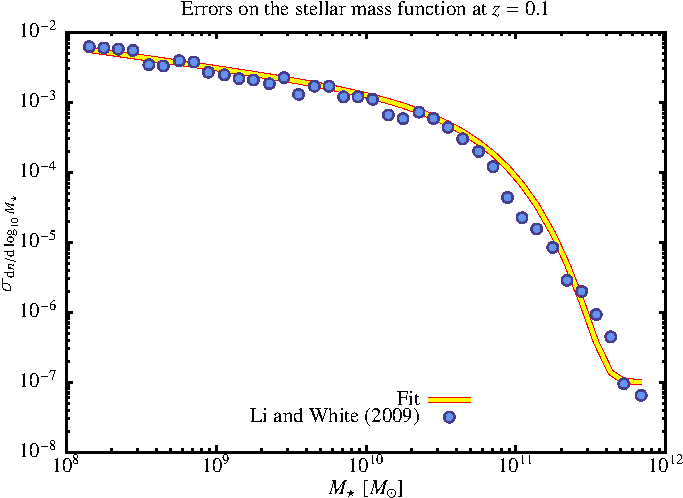
\includegraphics[width=160mm]{../plots/stellarMassFunctionErrors_z01.pdf}
 \end{center}
 \caption{Errors on the \protect\cite{li_distribution_2009} stellar mass funtion (points) and the fitting function (line) given by eqn.~(\protect\ref{eq:stellarMassFunctionErrorsFit}).}
 \label{fig:stellarMassFunctionErrors}
\end{figure}

\begin{figure}
 \begin{center}
 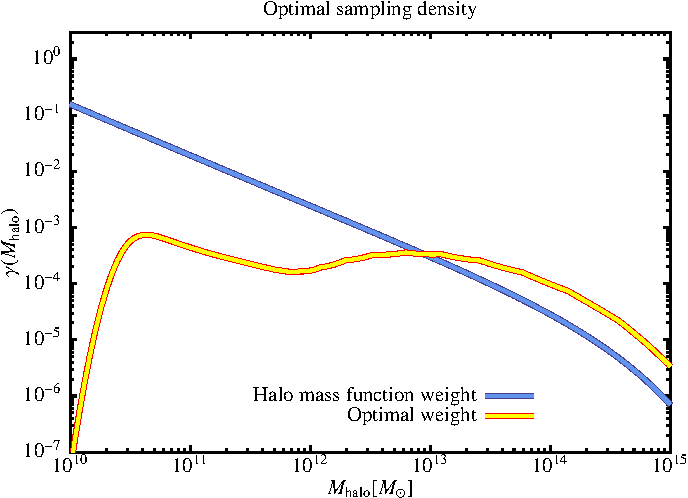
\includegraphics[width=160mm]{../plots/optimalSamplingStellarMassFunction.pdf}
 \end{center}
 \caption{Optimal weighting (yellow line) compared with weighting by the dark matter halo mass function (i.e. sampling halos at random from a representative volume; blue line). Sampling densities have been normalized to unit compute time.}
 \label{fig:optimalSamplingStellarMassFunction}
\end{figure}

\subsection{Refining by Other Merger Tree Statistics}

Since building merger trees is relatively fast, while solving the baryonic physics is slow it may be advantageous to  non-uniformly sample the distribution of merger trees at fixed merger tree mass, $M$. For example, we could assign some measure of formation history to each merger tree, such as the time since the last major merger, $\tau$. The halo mass function then becomes $n(M,\tau)$ (which can be computed by simulating large numbers of trees), and the tree sampling function becomes $\gamma(M,\tau)$. We'd then need to know the stellar mass function conditioned on both $M$ and $\tau$, $\phi_\star(M_\star|M,\tau)$. Given these, the above approach could be easily generalized to determine an optimal $\gamma(M,\tau)$. Then, after generating a merger tree, we'd first compute $\tau$. If a sufficient number of trees in that $\tau$ interval had already been computed, then we'd simply drop that tree and compute another one. The speed up here would depend on how fast building trees is relative to solving baryonic physics and what fraction of trees you discard. In principle, the trees could be generated, sampled and stored in advance so that we'd already have an optimally distributed set of trees in $M$ and $\tau$ that could be used for each model run.

\section{Constraints}\label{sec:ConstraintScripts}

Any constraint which can be applied to \glc\ is defined by two files, a configuration file and a likelihood script, which must be placed in {\tt constraints/constraints} and {\tt constraints/scripts} respectively. 

\subsection{Configuration File}\label{sec:ConstraintConfigFiles}

The configuration file should have the form:
\begin{verbatim}
<!-- Defines a constraint to match some data. -->                                          
<constraint>                                                                                                         
  <name>Long-form name of this constraint</name>                                                                      
  <label>shortLabelForThisConstraint</label>                                                                        
  <outputRedshift>0.07</outputRedshift>                                                                              
  <outputRedshift>1.00</outputRedshift>                                                                              
  <haloMassResolution>5.0e9</haloMassResolution>                                                                     
  <haloMassMinimum>2.0e10</haloMassMinimum>                                                                          
  <haloMassMaximum>2.0e14</haloMassMaximum>                                                                          
  <analysis>constraints/scripts/myAnalysisScript.pl</analysis>                                         
  <luminosity>
    <filter>UKIRT_K</filter>
    <redshift>0.0</redshift>
    <frame>rest</frame>
  </luminosity>
  <luminosity>
    <filter>UKIRT_K</filter>
    <redshift>1.0</redshift>
    <frame>observed</frame>
  </luminosity>
  <optionOn>outputMainBranchStatus</optionOn>
  <optionOn>outputDensityContrastData</optionOn>
  <parameter>
   <name>outputDensityContrastValues</name>
   <value>200.0</value>
   <accumulation>unique</accumulation>
  </parameter>
</constraint>                                                                                                        
\end{verbatim}
The {\tt name} and {\tt label} are used to describe the constraint ({\tt label} is used as a suffix in file names so should not contain spaces or other characters which might cause problems in file names). 

The remaining elements describe the requirements for this constraint. {\tt haloMassResolution} specifies the maximum resolution in mergers trees that still allows this constraint to be computed accurately. Similarly, {\tt haloMassMinimum} and {\tt haloMassMaximum} specify the required range of halo masses to simulate to allow this constraint to be computed accurately.

One or more {\tt outputRedshift} elements may be present, each specifying a redshift at which output is required for this constraint. Similarly, one or more {\tt luminosity} elements may be present, each of which specifies a luminosity which must be computed for this constraint. Each {\tt luminosity} must contain a specification of {\tt filter}, {\tt redshift}, and {\tt frame} to define which luminosity is to be computed.

One or more {\tt optionOn} elements may be present. Each element must specify the name of a \glc\ input parameter. That parameter will be set to {\tt true} in the \glc\ input parameter file.

Finally, arbitrary other parameter may be set using the standard {\tt parameter} element which should give the {\tt name} and {\tt value} for the parameter. Optionally, an {\tt accumulation} element may also be specified for each {\tt parameter}. This controls how values of the parameter are to be accumulated if set by more than one constraint. An accumulation of {\tt overwrite} will simply overwrite any previously set values. An accumulation of {\tt combine} will concatenate all values set by different constraints. Finally, an accumulation of {\tt unique} will concatenate all values set by different constraints and then filter out any duplicates.

When multiple constraints are used, their requirements are automatically combined.

\subsection{Likelihood Script}

The likelihood script for a constraint is required to perform several tasks, controlled by command line options. The script should accept the following command line syntax:
\begin{verbatim}
 myScript.pl <galacticusFile> [options...]
\end{verbatim}
where {\tt galacticusFile} is the file name of the \glc\ model for which the likelihood calculation should be performed. The following options must be supported by the script:
\begin{description}
 \item [{\tt --plotFile <fileName>}] If this option is present, the script should generate a plot showing the constraint and the model result and write it to {\tt fileName}.
 \item [{\tt --outputFile <fileName>}] If this option is present, the script should compute the log-likelihood of the model given the constraint and write it to {\tt fileName} using the format
\begin{verbatim}
 <constraint>
  <logLikelihood>-123</logLikelihood>
 </constraint>
\end{verbatim}
 \item [{\tt --accuracyFile <fileName>}] If this option is present, the script should write an XML file giving details of the accuracy of the model results relative to the observational errors using the format
\begin{verbatim}
 <accuracy>
  <x>...</x>
  .
  .
  .
  <x>...</x>
  <yModel>...</yModel>
  .
  .
  .
  <yModel>...</yModel>
  <yData>...</yData>
  .
  .
  .
  <yData>...</yData>
  <errorModel>...</errorModel>
  .
  .
  .
  <errorModel>...</errorModel>
  <errorData>...</errorData>
  .
  .
  .
  <errorData>...</errorData>
 </accuracy>
\end{verbatim}
In this file the {\tt yModel} and {\tt yData} elements should give the values of the model result and the comparable data respectively, while {\tt errorModel} and {\tt errorData} should give an estimate of the errors on these quantities. In the case of the model error this should include only the contribution arising from the finite number of merger trees simulated. This file will be used to judge whether the model is running sufficient merger trees such that the likelihood is not dominated by these errors. The {\tt x} elements are optional but can be used to give the parameter values associated with each model result.
 \item [{\tt --resultFile <fileName>}] If this option is present, the script should write an XML file giving details of the result of the model using the format
\begin{verbatim}
 <accuracy>
  <x>...</x>
  .
  .
  .
  <x>...</x>
  <y>...</y>
  .
  .
  .
  <y>...</y>
  <error>...</error>
  .
  .
  .
  <error>...</error>
 </accuracy>
\end{verbatim}
In this file the {\tt y} elements should give the values of the model result, while the {\tt error} elements should give an estimate of the errors on these results. The error should include only the contribution arising from the finite number of merger trees simulated. This file will be used to judge whether the model result is converged with respect to various numerical parameters in \glc. The {\tt x} elements are optional but can be used to give the parameter values associated with each model result.
 \item [{\tt --modelDiscrepancies <path>}] If this option is present, the script should scan {\tt path}. For each directory found in {\tt path} the script should check for the existance of a file named {\tt discrepancy<label>.hdf5} where {\tt label} is the label given for this constraint in its configuration file (see \S\ref{sec:ConstraintConfigFiles}). If present, the model discrepancy given in that file should be applied to the likelihood calculation. See \S\ref{sec:ModelDiscrepancy} for a description of the structure of the discrepancy files.
\end{description}

\subsection{Available Constraints}

\subsubsection{Li \& White (2009) SDSS Stellar Mass Function}

This constraint utilizes the stellar mass function for $z\approx 0.07$ galaxies measured by \cite{li_distribution_2009} from the \gls{sdss}. The mass function reported by \cite{li_distribution_2009} is converted to the appropriate Hubble constant for the given \glc\ model (assuming that masses scale as $H_0^{-2}$ and volumes as $H_0^3$)---no adjustment is made for cosmological parameters given the low redshift of the sample.

Given a \glc\ model, total stellar masses of model galaxies are adjusted using:
\begin{equation}
 M_\star \rightarrow {\bf G} {\bf S} M_\star 
\end{equation}
where the ${\bf S}$ operator is a multiplicative factor accounting for systematic errors in stellar mass determination and is equal to \citep{behroozi_comprehensive_2010}
\begin{equation}
 \log_{\rm 10} S = \mu + \kappa \log_{\rm 10} \left({M_\star \over 10^{11.3}M_\odot}\right)
\end{equation}
where $\mu=${\tt [sdssStellarMassFunctionZ0.07StellarMassSystematicMu]}, $\kappa=${\tt [sdssStellarMassFunctionZ0.07StellarMassSystematiKappa]}, and the {\bf G} operator is a multiplicative factor drawn from a log-normal distribution of width $0.07$~dex for each galaxy to mimic the effects of random errors on stellar masses (motivated by the discussion of \cite{behroozi_comprehensive_2010}).

The model masses are then used to construct a mass function by binning into a histogram using the masses reported by \cite{li_distribution_2009} (modified as described above) as the centers of the bins (with bin boundaries placed at the geometric means of consecutive bin centers).

If the {\tt --modelDiscrepancies} option is given, then any multiplicative or additive discrepancies found are applied to the model mass function, and any additional covariance is added to the covariance matrix.

The covariance matrix is computed as
\begin{equation}
 {\bf C} = {\bf C}_{\rm obs} + {\bf C}_{\rm model,random} + \sum_i {\bf C}_{{\rm discrepancy}, i},
\end{equation}
where ${\bf C}_{\rm obs}$ is the covariance matrix of the observational data, ${\bf C}_{\rm model,random}$ is the covariance matrix of the model arising from random noise (due to the finite number of trees simulated---see \S\ref{sec:AnalysisALFALFAHIMassFunction} for a description of how this covariance matrix is estimated), and ${\bf C}_{{\rm discrepancy}, i}$ is the covariance due to the $i^{\rm th}$ model discrepancy.

The model likelihood is then computed using:
\begin{equation}
 \mathcal{L} = {1 \over \sqrt{(2 \pi)^n |{\bf C}|}} \exp\left[ -{1\over 2} \Delta {\bf C}^{-1} \Delta \right],
\end{equation}
where $\Delta_i = \Phi_{{\rm model}, i} - \Phi_{{\rm observed}, i}$ is the difference between the model and observed mass functions, and $n$ is the number of points in the mass function histogram.

Computing the large-scale structure contribution to the covariance function requires integration of the non-linear matter power spectrum over the Fourier transform of the survey window function. We use the method of \cite{peacock_non-linear_1996} to determine the non-linear matter power spectrum, because of its simplicity and speed. We have checked that using a more accurate non-linear matter power spectrum (e.g. \citealt{lawrence_coyote_2010}) makes negligible difference to our results.

To find a suitable \gls{hod} to describe the galaxies in the \cite{li_distribution_2009} sample we adopt the model of \cite{behroozi_comprehensive_2010}. This is an 11 parameter model which describes separately the numbers of satellite and central galaxies occupying a halo of given mass---the reader is referred to \cite{behroozi_comprehensive_2010} for a complete description of the functional form of this parametric \gls{hod}. 

To reproduce the mass function of \cite{li_distribution_2009} using this \gls{hod} we use the \gls{bie} \citep{weinberg_computational_2012} to constrain the \gls{hod} parameters. We use a likelihood
\begin{equation}
 \ln \mathcal{L} = -{1\over 2} \Delta\cdot \mathcal{C}^{-1}\cdot \Delta^{\rm T} - {N \over 2} \ln(2\pi) - {\ln |\mathcal{C}| \over 2},
\end{equation}
where $N$ is the number of bins in the mass function, $\mathcal{C}$ is the covariance matrix of the observed mass function, and $\Delta_i = \phi_i^{\rm (HOD)} - \phi_i^{\rm (observed)}$. Of course, it is precisely this covariance matrix, $\mathcal{C}$, that we are trying to compute. We therefore adopt an iterative approach as follows:
\begin{enumerate}
 \item make an initial estimate of the covariance matrix, assuming that only Poisson errors contribute (the covariance matrix is therefore diagonal, and the terms are easily computed from the measured mass function and the survey volume as a function of stellar mass);
 \item find the maximum likelihood parameters of the \gls{hod} given the observed mass function and the current estimate of the covariance matrix;
 \item using this \gls{hod} and the framework of \cite{smith_how_2012}, compute a new estimate of the covariance matrix, including all three contributions;
 \item repeat steps 2 and 3 until convergence in the covariance matrix is achieved.
\end{enumerate}
In practice we find that this procedure leads to an \gls{hod} and covariance matrix which oscillate between two states in successive iterations. The differences in the covariance matrix are relatively small however, so we choose to conservatively adopt the covariance matrix with the larger values. In future, adding additional constraints to the \gls{hod} (as described below) should help mitigate this problem.

\subsubsection{Martin et al. (2010) ALFALFA HI Mass Function}\label{sec:AnalysisALFALFAHIMassFunction}

This constraint utilizes the HI mass function for $z\approx 0.0$ galaxies measured by \cite{martin_arecibo_2010} from the ALFALFA survey. The mass function reported by \cite{martin_arecibo_2010} is converted to the appropriate Hubble constant for the given \glc\ model (assuming that masses scale as $H_0^{-2}$ and volumes as $H_0^3$)---no adjustment is made for cosmological parameters given the low redshift of the sample.

Given a \glc\ model, total gas masses of model galaxies are adjusted using:
\begin{equation}
 M_{\rm HI} \rightarrow {\bf G} {\bf S} M_{\rm gas}
\end{equation}
where the ${\bf S}$ operator is a multiplicative factor accounting for systematic errors in HI mass determination and for the unknown molecular fraction and is equal to:
\begin{equation}
 \log_{\rm 10} S = \mu + \kappa \log_{\rm 10} \left({M_\star \over 10^9M_\odot}\right)
\end{equation}
where $\mu=${\tt [alfalfaHiMassFunctionZ0.00MolecularFractionMu]}, $\kappa=${\tt [alfalfaHiMassFunctionZ0.00MolecularFractionKappa]}, and the {\bf G} operator is a multiplicative factor drawn from a log-normal distribution. The width of this log-normal is determined from the combination of observational random errors on HI mass and scatter in the H$_2$/HI mass ratio at fixed total gas mass. Observational random errors on HI mass are taken from Fig.~19 of \cite{haynes_arecibo_2011}. We fit the magnitude of the error as a function of HI mass using a functional form:
\begin{equation}
 \sigma_{\rm obs} = a + \exp\left(-{\log_{10}(M_{\rm HI}/M_\odot)-b\over c}\right),
\end{equation}
where $\sigma_{\rm obs}$ is the error on $\log_{10}(M_{\rm HI}/M_\odot)$. We find a good fit using values of $a=0.100$, $b=5.885$, and $c=0.505$ as shown in Fig.~\ref{fig:ALFALFAErrorModel}. 

\begin{figure}
 \begin{center}
 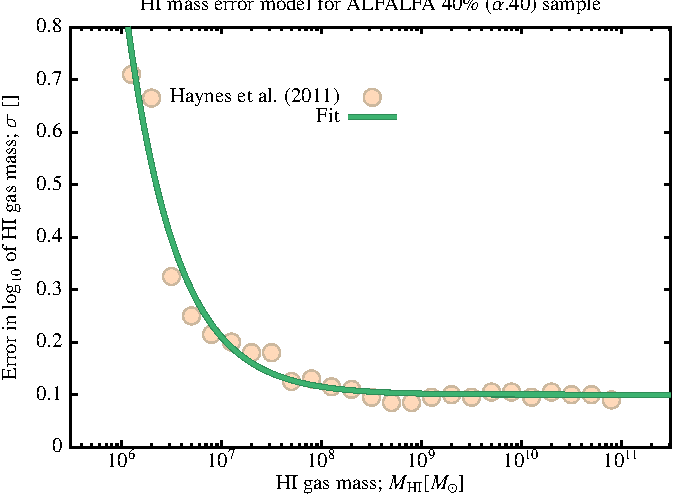
\includegraphics[width=85mm,trim=0mm 0mm 0mm 4mm,clip]{Plots/DataAnalysis/alfalfaHIMassErrorModel.pdf}
 \caption{The observational random error in galaxy HI mass as a function of HI mass for the ALFALFA survey. Points show the errors reported by \protect\cite{haynes_arecibo_2011}, while the line shows a simple functional form fit to these errors.}
 \end{center}
 \label{fig:ALFALFAErrorModel}
\end{figure}

In addition, we expect there to be significant scatter in the H$_2$/HI mass ratio at fixed total gas mass. For example, Figure~5 of \cite{power_redshift_2010} shows a broad distribution of such values. We approximate this scatter as a Gaussian random process with standard deviation $\sigma$. This random ``error'' is added in quadrature to the observational errors when constructing the mass function. For a prior on $\sigma$ we adopt a normal distribution with mean of $0.4$ (estimated from Figure~5 of \cite{power_redshift_2010}) and standard deviation $0.3$.

The model masses are then used to construct a mass function by binning into a histogram using the masses reported by \cite{martin_arecibo_2010} (modified as described above) as the centers of the bins (with bin boundaries placed at the geometric means of consecutive bin centers).

If the {\tt --modelDiscrepancies} option is given, then any multiplicative or additive discrepancies found are applied to the model mass function, and any additional covariance is added to the covariance matrix.

The covariance matrix is computed as
\begin{equation}
 {\bf C} = {\bf C}_{\rm obs} + {\bf C}_{\rm model,random} + \sum_i {\bf C}_{{\rm discrepancy}, i},
\end{equation}
where ${\bf C}_{\rm obs}$ is the covariance matrix of the observational data, ${\bf C}_{\rm model,random}$ is the covariance matrix of the model arising from random noise (due to the finite number of trees simulated, and ${\bf C}_{{\rm discrepancy}, i}$ is the covariance due to the $i^{\rm th}$ model discrepancy.

To construct ${\bf C}_{\rm model,random}$ we make use of the fact that \glc\ works by sampling a set of tree ``root masses'' from the $z=0$ dark matter halo mass function. From each root, a tree is grown, within which the physics of galaxy formation is then solved. Root masses are sampled uniformly from the halo mass function. That is, the cumulative halo mass function, $N(M)$, is constructed between the maximum and minimum halo masses to be simulated. The number of root masses, $N_{\rm r}$, to be used in a model evaluation is then determined. Root masses are then chosen such that
\begin{equation}
 N(M_i) = N(M_{\rm min}) {i-1 \over N_{\rm r}-1}
\end{equation}
for $i=1\ldots N_{\rm r}$ (noting that $N(M_{\rm max})=0$ by construction). 

Consider first those galaxies which form in the main branch of each tree (i.e. those galaxies which are destined to become the central galaxy of the $z=0$ halo). Suppose that we simulate $N_k$ halos of root mass $M_k$ at $z=0$. In such halos the main branch galaxies will, at any time, have stellar masses drawn from some distribution $p_k(M_\star|t)$. The number of such galaxies contributing to bin $i$ of the mass function is therefore binomially distributed with success probability $p_{ik} = \int_{M_{i,\rm min}}^{M_{i,\rm max}} p_k(M_\star|t) \d M_\star$ and a sample size of $N_k$. The contribution to the covariance matrix from these main branch galaxies is therefore:
\begin{equation}
 \mathcal{C}_{ij} = \left\{ \begin{array}{ll} p_{ik}(1-p_{ik}) N_k w_k^2 & \hbox{ if } i = j \\ -p_{ik} p_{jk} N_k w_k^2 & \hbox{ otherwise,} \end{array} \right.
\end{equation}
where $w_k$ is the weight to be assigned to each tree. To compute this covariance requires knowledge of the probabilities, $p_{ik}$. We estimate these directly from the model. To do this, we bin trees into narrow bins of root mass and assume that $p_{ik}$ does not vary significantly across the mass range of each bin. Using all realizations of trees that fall within a given bin, $k$, we can directly estimate $p_{ik}$.

In addition to the main branch galaxies, each tree will contain a number of other galaxies (these will be ``satellite'' galaxies at $z=0$, but at higher redshifts may still be central galaxies in their own halos). Tests have established that the number of satellites in halos is well described by a Poisson process. Note that each galaxy contributes Gaussian distribution to the mass function due to modelling of random errors in stellar mass determinations. For main branch galaxies this is simply accounted for when accumulating the probabilities, $p_{ik}$. For satellite galaxies, off-diagonal contributions to the covariance matrix arise as a result, $C_{ij} = w_k f_i f_j$, where $f_i$ is the fraction of the galaxy contributing to bin $i$ of the mass function.

The model likelihood is then computed using:
\begin{equation}
 \mathcal{L} = {1 \over \sqrt{(2 \pi)^n |{\bf C}|}} \exp\left[ -{1\over 2} \Delta {\bf C}^{-1} \Delta \right],
\end{equation}
where $\Delta_i = \Phi_{{\rm model}, i} - \Phi_{{\rm observed}, i}$ is the difference between the model and observed mass functions, and $n$ is the number of points in the mass function histogram.

Computing the large-scale structure contribution to the covariance function requires integration of the non-linear matter power spectrum over the Fourier transform of the survey window function. We use the method of \cite{peacock_non-linear_1996} to determine the non-linear matter power spectrum, because of its simplicity and speed. We have checked that using a more accurate non-linear matter power spectrum (e.g. \citealt{lawrence_coyote_2010}) makes negligible difference to our results.

To find a suitable \gls{hod} to describe the galaxies in the \cite{martin_arecibo_2010} sample we adopt the model of \cite{behroozi_comprehensive_2010}. This is an 11 parameter model which describes separately the numbers of satellite and central galaxies occupying a halo of given mass---the reader is referred to \cite{behroozi_comprehensive_2010} for a complete description of the functional form of this parametric \gls{hod}. 

To reproduce the mass function of \cite{martin_arecibo_2010} using this \gls{hod} we use the \gls{bie} \citep{weinberg_computational_2012} to constrain the \gls{hod} parameters. We use a likelihood
\begin{equation}
 \ln \mathcal{L} = -{1\over 2} \Delta\cdot \mathcal{C}^{-1}\cdot \Delta^{\rm T} - {N \over 2} \ln(2\pi) - {\ln |\mathcal{C}| \over 2},
\end{equation}
where $N$ is the number of bins in the mass function, $\mathcal{C}$ is the covariance matrix of the observed mass function, and $\Delta_i = \phi_i^{\rm (HOD)} - \phi_i^{\rm (observed)}$. Of course, it is precisely this covariance matrix, $\mathcal{C}$, that we are trying to compute. We therefore adopt an iterative approach as follows:
\begin{enumerate}
 \item make an initial estimate of the covariance matrix, assuming that only Poisson errors contribute (the covariance matrix is therefore diagonal, and the terms are easily computed from the measured mass function and the survey volume as a function of stellar mass);
 \item find the maximum likelihood parameters of the \gls{hod} given the observed mass function and the current estimate of the covariance matrix;
 \item using this \gls{hod} and the framework of \cite{smith_how_2012}, compute a new estimate of the covariance matrix, including all three contributions;
 \item repeat steps 2 and 3 until convergence in the covariance matrix is achieved.
\end{enumerate}
In practice we find that this procedure leads to an \gls{hod} and covariance matrix which oscillate between two states in successive iterations. The differences in the covariance matrix are relatively small however, so we choose to conservatively adopt the covariance matrix with the larger values. In future, adding additional constraints to the \gls{hod} (as described below) should help mitigate this problem.

\subsubsection{Shen et al. (2003) Late-Type Galaxy Size Distribution}\label{sec:SDSSLateTypeGalaxySizeDistribution}

This constraint utilizes the distribution of Petrosian half-light radii for $z\approx 0.07$ late-type galaxies measured by \cite{shen_size_2003} from the \gls{sdss}. The size function reported by \cite{shen_size_2003} is converted to the appropriate cosmology for the given \glc\ model (assuming that sizes scale as the angular diameter distance, and masses as the square of the luminosity distance).

Given a \glc\ model, total stellar masses of model galaxies are adjusted using:
\begin{equation}
 M_\star \rightarrow {\bf G} {\bf S} M_\star 
\end{equation}
where the ${\bf S}$ operator is a multiplicative factor accounting for systematic errors in stellar mass determination and is equal to \citep{behroozi_comprehensive_2010}
\begin{equation}
 \log_{\rm 10} S = \mu + \kappa \log_{\rm 10} \left({M_\star \over 10^{11.0}M_\odot}\right)
\end{equation}
where $\mu=${\tt [diskGalaxySizesSDSSZ0.07MassSystematic0]}, $\kappa=${\tt [diskGalaxySizesSDSSZ0.07MassSystematic1]}, and the {\bf G} operator is a multiplicative factor drawn from a log-normal distribution of width $0.0806$~dex for each galaxy to mimic the effects of random errors on stellar masses (motivated by the statement from \cite{shen_size_2003} who quote the 95\% confidence
interval on masses as being $\pm 40$\%).

{\bf Note:} This analysis currently assumes that model galaxies have disk Petrosian half-mass radii of
\begin{equation}
 R_{\rm 50} = 1.6676 {1 \over \sqrt{2}} \lambda R_{\rm vir}.
\end{equation}

Disk sizes of model galaxies are then adjusted using:
\begin{equation}
 R_{50} \rightarrow {\bf G} {\bf S} R_{50} 
\end{equation}
where the ${\bf S}$ operator is a multiplicative factor accounting for systematic errors in radius determination and in determination of radius from halo virial radius and spin and is equal to
\begin{equation}
 \log_{\rm 10} S = \mu + \kappa \log_{\rm 10} \left({R_{50} \over 1 \hbox{kpc}}\right)
\end{equation}
where $\mu=${\tt [iskGalaxySizesSDSSZ0.07RadiusSystematic0]}, $\kappa=${\tt [iskGalaxySizesSDSSZ0.07RadiusSystematic1]}, and the {\bf G} operator is a multiplicative factor drawn from a log-normal distribution of width $0.0128$~dex for each galaxy to mimic the effects of random errors on disk radii (estimated from the fractional errors reported in the \gls{sdss} database).

The model sizes and masses are then used to construct a mass-dependent radius function by binning into a 2-D histogram using the size and mass bins reported by \cite{shen_size_2003} (modified as described above) as the centers of the bins (with bin boundaries placed at the geometric means of consecutive bin centers).

If the {\tt --modelDiscrepancies} option is given, then any multiplicative or additive discrepancies found are applied to the model mass function, and any additional covariance is added to the covariance matrix.

The covariance matrix is computed as
\begin{equation}
 {\bf C} = {\bf C}_{\rm obs} + {\bf C}_{\rm model,random} + \sum_i {\bf C}_{{\rm discrepancy}, i},
\end{equation}
where ${\bf C}_{\rm obs}$ is the covariance matrix of the observational data, ${\bf C}_{\rm model,random}$ is the covariance matrix of the model arising from random noise (due to the finite number of trees simulated, and ${\bf C}_{{\rm discrepancy}, i}$ is the covariance due to the $i^{\rm th}$ model discrepancy.

The model covariance matrix is estimated using the sample methods as described in \S\ref{sec:AnalysisALFALFAHIMassFunction}. The only difference is that in this case we have a 2-D histogram. This 2-D histogram is ``flattened'' into a 1-D vector for purposes of likelihood computation however, so covariance matrix estimation proceeds unchanged. (Note that correlations between mass bins are accounted for, in additional to correlations between radius bins.) Since the radius functions of \cite{shen_size_2003} are normalized to unity at each mass, we must account for this in the covariance matrix. The radius function transforms as:
\begin{equation}
 f_{ik} \rightarrow {f_{ik} \over \Delta \log_{10} R \sum_i f_{ik} },
\end{equation}
where $i$ indexes radius bins, $k$ indexes mass bins, and $\Delta \log_{10} R$ is the width of the radius bin. The Jacobian of this transformation is simply
\begin{equation}
 J_{ij} = {\delta_{ij} - f_i \over  \Delta \log_{10} R \sum_i f_{ik}}.
\end{equation}
Therefore, the covariance matrix is modified according to $\mathcal{C} \rightarrow J \mathcal{C} J^{\rm T}$. The same transformation is applied to the covariance matrix of the observed data (for which the reported errors are simply the Poisson errors on each bin).

The model likelihood is then computed using:
\begin{equation}
 \mathcal{L} = {1 \over \sqrt{(2 \pi)^n |{\bf C}|}} \exp\left[ -{1\over 2} \Delta {\bf C}^{-1} \Delta \right],
\end{equation}
where $\Delta_i = \Phi_{{\rm model}, i} - \Phi_{{\rm observed}, i}$ is the difference between the model and observed mass functions, and $n$ is the number of points in the mass function histogram.

\section{Constraint Compilations}

To specify which constraints will be applied to a particular model, a compilation file is used. These must be stored in {\tt constraints/compilations}. An example of such a file follows:
\begin{verbatim}
<constraintCompilation>
  <constraint>
    <definition>constraints/constraints/stellarMassFunction_SDSS_z0.07.xml</definition>
    <weight>1.0</weight>
  </constraint>
  <constraint>
    <definition>constraints/constraints/hiMassFunction_ALFALFA_z0.00.xml</definition>
    <weight>1.0</weight>
  </constraint>
</constraintCompilation>
\end{verbatim}
Each {\tt constraint} element specifies one constraint that will be included in this compilation, and must contain a {\tt definition} element, giving the path of the configuration file for this constraint, and a {\tt weight} element which allows the relative weight given to each constraint to be varied\footnote{Note that, if your constraints are computing correct likelihoods, re-weighting them may not be a good idea. \emph{Caveat constrainor.}}.

\section{Constraint File}

\glc\ has a complete constraints infrastructure which implements various \gls{mcmc} algorithms to analyze the posterior probability distribution of the model given some compilation of constraints. The infrastructure is \gls{mpi} parallelized and ideal for running on large compute clusters.

To perform a constraint calculation simply build the constraint code:
\begin{verbatim}
 make Constrain_Galacticus.exe
\end{verbatim}
and run with a parameter file and configuration file. Typically, you will want to run this code under \gls{mpi}, for example:
\begin{verbatim}
 mpirun -n 4 Constrain_Galacticus.exe mcmcParameters.xml mcmcConfig.xml
\end{verbatim}
would run 4 processes (typically you will need to run many more than this). If running on a \gls{pbs} queue, embed this command in a suitable \gls{pbs} script and submit. 

The parameter file follows the same format as a standard \glc\ parameter file and specifies the values of parameters to be used. For example, the seed used fo pseudo-random number sequences can be specified in this file. 

The configuration file specifies the details of the constraint simulation to be performed. An example configuration file is:
\begin{verbatim}
<?xml version="1.0" encoding="UTF-8"?>
<simulationConfig>

  <likelihood>
    <type>Galacticus</type>
    <name>verySimplisticToStellarMassFunction</name>
    <compilation>stellarMassFunction_SDSS_z0.07.xml</compilation>
    <baseParameters>./mcmcWork/verySimplisticToStellarMassFunctionBase.xml</baseParameters>
    <workDirectory>./mcmcWork</workDirectory>
    <scratchDirectory>./mcmcScratch</scratchDirectory>
    <report>no</report>
    <randomize>no</randomize>
    <threads>4</threads>
    <saveState>no</saveState>
    <cpulimit>1200</cpulimit>
    <memoryLimit>2gb</memoryLimit>
    <environment>LD_LIBRARY_PATH=/opt/gcc-trunk/lib:/opt/gcc-trunk/lib64:/usr/local/upstream/lib:$LD_LIBRARY_PATH</environment>
    <environment>PATH=/opt/gcc-trunk/bin:$PATH</environment>
    <environment>GFORTRAN_ERROR_DUMPCORE=NO</environment>
  </likelihood>

  <convergence>
    <type>GelmanRubin</type>
    <Rhat>1.2</Rhat>
    <burnCount>100</burnCount>
    <testCount>100</testCount>
    <outlierCountMaximum>0</outlierCountMaximum>
    <outlierSignificance>0.95</outlierSignificance>
    <outlierLogLikelihoodOffset>60</outlierLogLikelihoodOffset>
  </convergence>
  
  <state>
    <type>history</type>
    <acceptedStateCount>100</acceptedStateCount>
  </state>
  
  <proposalSize>
    <type>adaptive</type>
    <gammaInitial>1.77</gammaInitial>
    <gammaFactor>1.414</gammaFactor>
    <acceptanceRateMinimum>0.4</acceptanceRateMinimum>
    <acceptanceRateMaximum>0.6</acceptanceRateMaximum>
    <updateCount>10</updateCount>
  </proposalSize>
  
  <randomJump>
    <type>adaptive</type>
  </randomJump>
  
  <simulation>
    <type>temperedDifferentialEvolution</type>
    <stepsMaximum>1000000</stepsMaximum>
    <stepsPostConvergence>100000</stepsPostConvergence>
    <acceptanceAverageCount>100</acceptanceAverageCount>
    <logFileRoot>./mcmcWork/mcmc/chains</logFileRoot>
    <temperatureMaximum>64.0</temperatureMaximum>
    <untemperedStepCount>20</untemperedStepCount>
    <temperedLevels>10</temperedLevels>
    <stepsPerLevel>10</stepsPerLevel>
  </simulation>

  <parameters>
    <parameter>
      <name>starFormationTimescaleDisksHaloScalingVirialVelocityExponent</name>
      <prior>
	<distribution>
	  <type>uniform</type>
	  <minimum>-6.0</minimum>
	  <maximum>+0.0</maximum>
	</distribution>
      </prior>
      <random>
	<type>Cauchy</type>
	<median>0.0</median>
	<scale>0.006</scale>
      </random>
    </parameter>
    <parameter>
      <name>starFormationTimescaleDisksHaloScalingRedshiftExponent</name>
      <prior>
	<distribution>
	  <type>uniform</type>
	  <minimum>-1.0</minimum>
	  <maximum>+4.0</maximum>
	</distribution> 
      </prior>
      <random>
	<type>Cauchy</type>
	<median>0.0</median>
	<scale>0.005</scale>
      </random>
    </parameter>
  </parameters>
  
</simulationConfig>
\end{verbatim}

The following subsections describe each entry in this file.

\subsection{{\tt likelihood}}

The {\tt likelihood} section specifies the likelihood function to be used in the simulation. The type of likelihood to use is specified by the {\tt type} element. The available choices are described in the following subsections.

\subsubsection{multivariateNormal}

The likelihood is a simple multivariate Gaussian, intended primarily for testing purposes. The distribution parameters are specified within the {\tt likelihood} element using:
\begin{verbatim}
  <mean>0.45 0.50</mean>
  <covariance>
    <row>1.0e-4 -0.9e-4</row>
    <row>-0.9e-4 1.0e-4</row>
  </covariance>
\end{verbatim}
where the {\tt mean} element gives the mean vector of $N$ elements, and the {\tt covariance} element contains $N$ {\tt row} elements each containing a vector of $N$ elements giving a single row of the covariance matrix. The likelihood is then:
\begin{equation}
\log \mathcal{L} = - {1 \over 2} \Delta \mathcal{C}^{-1} \Delta^{\rm T},
\end{equation}
where $Delta = \theta - \bar{\theta}$, $\theta$ is the state, $\bar{\theta}$ is the mean, and $\mathcal{C}$ is the covariance matrix.

\subsubsection{Galacticus}

The likelihood is computed by running and analyzing a \glc\ model. The details of the model to run are specified by the follow content within the {\tt likelihood} element:
\begin{verbatim}
  <name>verySimplisticToStellarMassFunction</name>
  <compilation>stellarMassFunction_SDSS_z0.07.xml</compilation>
  <baseParameters>./mcmcWork/verySimplisticToStellarMassFunctionBase.xml</baseParameters>
  <workDirectory>./mcmcWork</workDirectory>
  <scratchDirectory>./mcmcScratch</scratchDirectory>
  <report>no</report>
  <randomize>no</randomize>
  <threads>4</threads>
  <saveState>no</saveState>
  <cpulimit>1200</cpulimit>
  <memoryLimit>2gb</memoryLimit>
  <environment>LD_LIBRARY_PATH=/opt/gcc-trunk/lib:/opt/gcc-trunk/lib64:/usr/local/upstream/lib:$LD_LIBRARY_PATH</environment>
  <environment>PATH=/opt/gcc-trunk/bin:$PATH</environment>
  <environment>GFORTRAN_ERROR_DUMPCORE=NO</environment>
\end{verbatim}

The entries have the following meanings:
\begin{description}
\item[{\tt name}] A name to use for this calculation. It will be used as the name for jobs submitted to the PBS queue for example.
\item[{\tt compilation}] Specifies the compilation file to be used for this analysis.
\item[{\tt baseParameters}] Specifies the path to a \glc\ parameter file which will be used as the base set of parameter on top of which any parameter variations will be applied.
\item[{\tt workDirectory}] The full path to a directory in which the results (e.g. \gls{mcmc} chains) will be stored.
\item[{\tt scratchDirectory}] The full path to a scratch directory where \glc\ model outputs and other temporary data will be written.
\item[{\tt report}] If set to {\tt yes}, reports additional debugging information during the run.
\item[{\tt randomize}] If {\tt yes} then each model evaluation will be performed with a different random number seed. Otherwise, the same seed is used in all cases. Experiment shows that changing the random number seed between evaluations can seriously limit the ability of \gls{mcmc} algorithms to converge.
\item[{\tt threads}] The number of parallel OpenMP threads to use for each \glc\ model. It is recommended that this be set to the number of available cores on each node, and semaphoring (see \S{sec:Semaphores}) be used. In this way, each copy of \glc\ on a node will share resources, but as one instance finishes, the others will be able to make use of the freed resources.
\item[{\tt saveState}] If {\tt yes} then \glc\ will save its internal state prior to beginning evolution of each merger tree. This is intended for debugging purposes and so should normally be set to {\tt no}.
\item[{\tt cpulimit}] A CPU time limit for each model evalulation. This can be useful if certain obscure regions of the surveyed parameter space result in unacceptably long run times. Models will be killed after this time and a very low likelihood returned.
\item[{\tt environment}] One of more such element can appear. Each specifies the value of an environment variable to be set prior to launching the \glc\ model.
\item[{\tt storeResults}] If {\tt yes} then the full results (e.g. the quantities computed to compare with observational data) from each model evalulation will be stored. Otherwise, they are discarded after each evalulation. Use {\tt yes} with caution---a typical run might include millions of model evaluations which can quickly lead to huge amounts of data being written to disk.
\end{description}

\subsection{{\tt convergence}}

The {\tt convergence} section specifies the criterion to be used to judge when the simulation has converged. The type of convergence criterion to use is specified by the {\tt type} element. The available choices are described in the following subsections.

\subsubsection{{\tt never}}

This option assumes that the simulation never converges, and so the calculation will run indefinitely. It is intended primarily for testing purposes.

\subsubsection{{\tt GelmanRubin}}

This option adopts the convergence criterion proposed by \citeauthor{gelman_a._inference_1992}~(\citeyear{gelman_a._inference_1992}; see also \citealt{brooks_general_1998}), which compares the variance in parameter values within chains to that between chains. Outlier detection is applied to the chains using a standard Grubb's outlier test. The behavior of this criterion is controlled by the following options which should be placed within the {\tt convergence} element:
\begin{description}
\item [{\tt Rhat}] The correlation coefficient, $\hat{R}$, value at which to declare convergence.
\item [{\tt burnCount}] Set number of steps to burn before applying the convergence test.
\item [{\tt testCount}] Set the number of steps between successive applications of the convergence test.
\item [{\tt outlierSignificance}] The significance level required in outlier detection.
\item [{\tt outlierLogLikelihoodOffset}] The offset in log-likelihood from the current maximum likelihood chain required for a chain to be declared to be an outlier.
\item [{\tt outlierCountMaximum}] The maximum number of outlier chains allowed.
\end{description}

\subsection{{\tt state}}

The {\tt state} section specifies the type of object used to record the state of the simulation. The type of state object to use is specified by the {\tt type} element. The available choices are described in the following subsections.

\subsubsection{{\tt simple}}

This type stores the current state but makes no attempt to record a history of the state and so cannot provide measures of the mean or variance of state over the simulation history. It does, however, maintain a running average of the state acceptance rate. The number of steps over which the acceptance rate should be computed is specified by the {\tt acceptedStateCount}.

\subsubsection{{\tt history}}

An extension of the {\tt simple} state, this type also records the mean and variance of each parameter over the history of the simulation.

\subsection{{\tt proposalSize}}

The {\tt proposalSize} section specifies the method to use when selecting the proposal size parameter, $\gamma$ (the fraction of the vector connecting to chain state to be used as the proposal for another chain), for use in differential evolution simulations. The proposal size algorithm to use is specified by the {\tt type} element. The available choices are described in the following subsections.

\subsubsection{{\tt fixed}}

This option uses a fixed $\gamma$ specified by the {\tt gamma} element.

\subsubsection{{\tt adaptive}}

This option adaptively changes $\gamma$ in an attempt to maintain the acceptance rate at an acceptable level. The algorithm is controlled by the following parameters (to be specified as elements within the {\tt proposalSize} element):
\begin{description}
\item[{\tt gammaInitial}] The initial value for $\gamma$.
\item[{\tt gammaFactor}] The multiplicative factor by which $\gamma$ should be increased or decreased if the acceptance rate is out of range.
\item[{\tt acceptanceRateMinimum}] The minimum acceptance rate to accept before reducing $\gamma$.
\item[{\tt acceptanceRateMaximum}] The maximum acceptance rate to accept before reducing $\gamma$.
\item[{\tt updateCount}] The number of steps between successive checks of the acceptance rate.
\end{description}

\subsection{{\tt randomJump}}

The {\tt randomJump} section specifies the method to use when adding a random jump component to proposals in differential evolution simulations. The random jump algorithm to use is specified by the {\tt type} element. The available choices are described in the following subsections.

\subsubsection{{\tt simple}}

The random jumps are drawn directly from the distributions specified in the {\tt random} element of each parameter (see \S\ref{sec:ParametersPriors}).

\subsubsection{{\tt adaptive}}

The random jumps are drawn from the distributions specified in the {\tt random} element of each parameter (see \S\ref{sec:ParametersPriors}) and then multiplied by the currently occupied range of each parameter (i.e. the maximum value of the parameter over all current chain states minus the minimum value of each parameter over all current chain states).

\subsection{{\tt simulation}}

The {\tt simulation} section specifies the algorithm to use to perform the simulation. The simulation algorithm to use is specified by the {\tt type} element. The available choices are described in the following subsections.

\subsubsection{{\tt differentialEvolution}}

This option uses the differential evolution algorithm of \cite{terr_braak_markov_2006}. Multiple, parallel chains are run and proposals are constructed by selecting two chains at random, taking a fraction, $\gamma$, of the vector connecting the two chain states and adding this to the state of the current chain. The details of the algorithm are controlled by the following elements which should be embedded within the {\tt simulation} element:
\begin{description}
\item[{\tt stepsMaximum}] The maximum number of steps to take.
\item[{\tt stepsPostConvergence}] The number of steps to perform after convergence is attained.
\item[{\tt acceptanceAverageCount}] The number of steps over which to average the acceptance rate.
\item[{\tt stateSwapCount}] The number of steps after which to set $\gamma=1$ to allow chains to swap states.
\item[{\tt logFileRoot}] The full path and root name of a file to log results to. The actual file name will have the rank of the \gls{mpi} process appended to it.
\end{description}

\subsubsection{{\tt temperedDifferentialEvolution}}

This option extends the {\tt differentialEvolution} option to include tempering during which the likelihood function is heated up and cooled down to allow chains to more easily walk through the likelihood landscape. In addition to the options for the {\tt differentialEvolution} algorithm, the details of the algorithm are controlled by the following elements whichy should be embedded within the {\tt simulation} element:
\begin{description}
\item[{\tt untemperedStepCount}] The number of untempered (i.e. $T=1$) steps to take between tempering cycles.
\item[{\tt temperatureMaximum}] The maximum temperature to use when tempering.
\item[{\tt temperedLevels}] The number of tempered levels to use.
\item[{\tt stepsPerLevel}] The number of differential evolution steps to take at each tempering level;
\item[{\tt gammaTemperatureExponent}] The exponent of the boost in $\gamma$ during tempered steps.
\end{description}

In each tempering cycle, the temperature is raised through levels $1$\ldots$N$ (where $N=${\tt temperedLevels}), and then back down through levels $N-1$\ldots$1$. The temperature at level $i$ is given by:
\begin{equation}
\log T_i = {i \over N} \log T_{\rm max},
\end{equation}
where $T_{\rm max}=${\tt temperatureMaximum}. During tempered steps, the $\gamma$ parameter of the differential evolution algorithm is increased by a factor $T^\alpha$, where $\alpha=${\tt gammaTemperatureExponent}. A value of $\alpha=1/2$ is optimal for a Gaussian likelihood.

\subsection{Parameters and Priors}\label{sec:ParametersPriors}

The {\tt parameters} section contains a list of all parameters to be varied in the analysis. Each parameter is described by one {\tt parameter} element. That element must contain a {\tt name} element, which gives the name of the parameter, a {\tt prior} element that contains a {\tt distribution} element defining the distribution for this prior, and (for differential evolution simulations) a {\tt random} element that defines the distribution to be used for the random perturbation to be added to this parameter in proposals.

\subsubsection{Loading External Parameters/Priors}

It is also possible to load parameters and their priors from external files. This is useful to add common sets of parameters, such as cosmological parameter. To do so, add an element of the form:
\begin{verbatim}
<xi:include href="../../constraints/parameters/wmap9Cosmology.xml" 
   xmlns:xi="http://www.w3.org/2001/XInclude" />
\end{verbatim}
\emph{after} the {\tt parameters} section of the constraint file. The {\tt href} attribute must give the path (relative to the constraint file, or absolute) to the external parameter file. This file should contain its own {\tt parameters} block, describing all parameters to be varied along with their priors. 

\subsubsection{Derived Parameter Values}

It is possible to define parameters in terms of other parameters. Common uses for this include:
\begin{itemize}
 \item Setting $\Omega_\Lambda$ from the value of $\Omega_{\rm M}$ to enforce a flat Universe;
 \item Setting the values of parameters with correlated priors as linear combinations of dummy parameters for which the priors are independent.
\end{itemize}
To define a parameter in this way include a {\tt parameter} element of the form:
\begin{verbatim}
<parameter>
 <name>sigma_8</name>
 <define>0.8178+%cosmology0*0.003817+%cosmology1*0.007931+%cosmology2*0.01002
    +%cosmology3*0.001584+%cosmology4*0.002931+%cosmology5*0.001727</define>
</parameter>
\end{verbatim}
Here the {\tt define} element gives an equation for the parameter in terms of other parameters. All standard mathematical operators and functions (as recognized by Perl) can be used, and other parameters referenced by using their name prefixed with a ``\%''.

\subsubsection{Including External Parameters}

Predefined sets of parameters (along with their priors) can be included using the {\tt xi:include} element. For example,
\begin{verbatim}
 <xi:include href="../../constraints/parameters/wmap7Cosmology.xml"
    xmlns:xi="http://www.w3.org/2001/XInclude" />
\end{verbatim}
will include a set of parameters from the file {\tt ../../constraints/parameters/wmap7Cosmology.xml} which defines priors on cosmological parameters consistent with the covariance matrix of the WMAP-7 cosmological constraints \citep{komatsu_seven-year_2010}.

\subsection{Distributions}

Various distribution functions (for priors and random perturbations) are supported. Where needed, the type of distribution should be specified in a {\tt type} element. Additional parameters of the distribution are specified using the elements described in the following subsections.

\subsubsection{{\tt uniform}}

A uniform distribution over a finite range
\begin{equation}
P(x) \propto \left\{ \begin{array}{ll} 1 & \hbox{ if } x_{\rm l} \leq x \leq x_{\rm u} \\ 0 & \hbox{ otherwise.}  \end{array} \right.
\end{equation}
Specified using:
\begin{description}
\item[{\tt minimum}] The lower limit of the range, $x_{\rm l}$;
\item[{\tt maximum}] The upper limit of the range, $x_{\rm u}$.
\end{description}

\subsubsection{{\tt logUniform}}

A distribution uniform in the logarithm of $x$ over a finite range
\begin{equation}
P(x) \propto \left\{ \begin{array}{ll} x^{-1} & \hbox{ if } x_{\rm l} \leq x \leq x_{\rm u} \\ 0 & \hbox{ otherwise.}  \end{array} \right.
\end{equation}
Specified using:
\begin{description}
\item[{\tt minimum}] The lower limit of the range, $x_{\rm l}$;
\item[{\tt maximum}] The upper limit of the range, $x_{\rm u}$.
\end{description}

\subsubsection{{\tt normal}}

A normal distribution, optionally with lower and upper limits:
\begin{equation}
P(x) \propto \left\{ \begin{array}{ll} \exp[-(x-\mu)^2/2S] & \hbox{ if } x_{\rm l} \leq x \leq x_{\rm u} \\ 0 & \hbox{ otherwise.}  \end{array} \right.
\end{equation}
Specified using:
\begin{description}
\item[{\tt mean}] The mean, $\mu$;
\item[{\tt variance}] The variance, $S$;
\item[{\tt minimum}] The lower limit of the range, $x_{\rm l}$;
\item[{\tt maximum}] The upper limit of the range, $x_{\rm u}$.
\end{description}

\subsubsection{{\tt Cauchy}}

A Cauchy distribution:
\begin{equation}
P(x) \propto \left[1+{x-x_0\over\gamma}\right]^{-1}.
\end{equation}
Specified using:
\begin{description}
\item[{\tt median}] The median, $x_0$;
\item[{\tt scale}] The scale, $\gamma$;
\end{description}

\subsubsection{{\tt StudentT}}

Student's t-distribution:
\begin{equation}
P(x) \propto \left(1 + {x^2\over \nu}\right)^{-(\nu+1)/2}
\end{equation}
Specified using:
\begin{description}
\item[{\tt degreesOfFreedom}] The number of degrees of freedom, $\nu$.
\end{description}
